\documentclass[10pt,a4paper]{article}
\usepackage[utf8]{inputenc}
\usepackage[italian]{babel}
\usepackage{amsmath}
\usepackage{amsfonts}
\usepackage{amssymb}
\usepackage{graphicx}
\usepackage{fullpage}
\usepackage{hyperref}
\usepackage{graphicx}
\usepackage{caption}
\usepackage{subcaption}

\author{Michele Carignani, Alessandro Lenzi}
\title{Analisi aggregata per ore}
\begin{document}

\maketitle

\section{Generazione dei grafi orari}

Per prima cosa i dati sono stati aggregati per ora. I dati originali del dataset 
%todo sistemare dataset
\href{https://dandelion.eu/datagem/telecom-mi-to-mi/description/}{Telecommunications - MI to MI} sono nel formato:
\begin{verbatim}
timestamp \t SourceId \t DestId \t Stregth
\end{verbatim}
e sono stati suddivisi in 24 file (uno per ogni ora) e aggregati, per cui
ogni file contiene (al massimo\footnote{poichè certi nodi possono non avere chiamate in uscita
in una certa fascia oraria.}) un record per ogni nodo nel formato:
\begin{verbatim}
SourceId \t DestId:Strength [\t DestId:Strength]
\end{verbatim}

A questo punto i pesi sugli archi (sopra chiamati \verb!Strength!) sono stati riscalati rispetto alla somma
dei valori della stella uscente di un nodo, ottenendo la probabilità di transire dal nodo $i$ al 
nodo $j$, ovvero:
$$ sumStrength_i = \sum_{j \in FS(i)} Strength_{ij} $$
$$ probability_{ij} = \frac{Strength_{ij}}{sumStrength_i} $$

\section{Ricerca delle componenti fortemente connesse}
Per effettuare la ricerca delle componenti fortemente connesse (in seguito CFC) è stato utilizzato l'algoritmo Tarjan, il cui pseudocodice (tratto da Wikipedia, \href{http://en.wikipedia.org/wiki/Tarjan''s_strongly_connected_components_algorithm}{Tarjan's Strongly Connected Components algorithm}) è mostrato in \ref{pseudotarjan}.
\begin{figure}
\begin{verbatim}
  input: graph G = (V, E)
  output: set of strongly connected components (sets of vertices)
  index := 0
  S := empty
  for each v in V do
    if (v.index is undefined) then
      strongconnect(v)
    end if
  end for

  function strongconnect(v)
    v.index := index
    v.lowlink := index
    index := index + 1
    S.push(v)
    for each (v, w) in E do
      if (w.index is undefined) then
        strongconnect(w)
        v.lowlink  := min(v.lowlink, w.lowlink)
      else if (w is in S) then
        v.lowlink  := min(v.lowlink, w.index)
      end if
    end for
    if (v.lowlink = v.index) then
      start a new strongly connected component
      repeat
        w := S.pop()
        add w to current strongly connected component
      until (w = v)
      output the current strongly connected component
    end if
  end function
\end{verbatim}
\caption{Pseudocodice dell'algoritmo di Tarjan per la ricerca delle CFC}
\label{pseudotarjan}
\end{figure}
L'approccio iniziale è stato quello di utilizzare una semplice visita ordinata sull'identificatore dell'arco (i.e. \texttt{for i = 0 to 10000 do strongconnect(i)}). Tale visita è stata effettuata con diversi tagli. In tutti i vari esperimenti, è stato possibile notare che l'ordine di visita dei nodi ha una notevole influenza sulle CFC trovate. Ad esempio, effettuando un taglio \emph{semplice} (per la spiegazione riguardo tagli si veda \ref{tagli}) al valore 0.005, si trova in pressoché tutte le ore una componente fortemente connessa molto grande, con nodi con valori nelle prime decine e che arrivano fino a 10000, per poi trovarne alcune altre estremamente piccole.
\'E evidente che in questo caso il taglio è estremamente basso, e perciò non necessariamente significativo: quello che invece viene messo in evidenza è che l'ordine di visita del grafo ha una notevole influenza sulle CFC individuate, come si può capire dal primo \texttt{for} nello pseudocodice in \ref{pseudotarjan}.

Il secondo passagio è stato dunque quello di ottenere una \textbf{strategia di visita} che potesse essere consistente con il traffico effettivo nella giornata.
Lo strumento al quale abbiamo pensato è stato quello di utilizzare un secondo dataset, ovvero \href{https://dandelion.eu/datagem/telecom-sms-call-internet-mi/description/}{"Telecommunications - SMS, Call, Internet - MI"}:
a partire dai record del formato
\begin{verbatim}
SquareID \t Timestamp \t .. ChiamateInUscita ..
\end{verbatim}
per ogni ora sono stati generati file con record.
\begin{verbatim}
SquareID \t AggregatedCalls
\end{verbatim}
Inoltre, è stato generato un ulteriore file in cui, per il giorno analizzato, viene mostrato il traffico totale uscente da ogni griglia, sempre nel formato di cui sopra.

I file generati sono stati dunque impiegati al fine della definizione di un ordinamento nella visita.
Il primo approccio è stato quello di compiere la visita con criteri diversi per ogni ora, per una cui analisi dettagliata si rimanda alla rispettiva sottosezione nel listato sottostante:
\begin{enumerate}
\item SCC1, visibile in \ref{SCC1sec} è una visita del grafo con nodi ordinati per \textbf{traffico orario crescente} e con archi della stella uscente selezionati per \textbf{probabilità crescente} 
\item SCC2 visita i nodi per \textbf{traffico orario decrescente} ordinando gli archi per \textbf{probabilità crescente}
\item SCC3 visita i nodi per \textbf{traffico orario decrescente} e gli archi per \textbf{probabilità decrescente}
\item SCC4 visita i nodi per \textbf{traffico orario crescente} e gli archi per \textbf{probabilità decrescente}
\end{enumerate}
Si noti come tale approccio in realtà si sia mostrato poco soddisfacente in tutti i quattro casi in analisi. Difatti, al fine della verifica di "persistenza" delle CFC individuate, una potenziale variazione di ordinamento nella visita avrebbe potuto comportare una distruzione delle CFC precedentemente individuate.

Il passo successivo è stato quindi quello di definire un ordinamento giornaliero sui nodi, al fine di effettuare delle visite possibilmente coerenti sui vari grafi orari generati. L'esperimento effettuato in questo caso può essere visto in \ref{stable3}

\subsection{Tagli}
\label{tagli}
I tagli sono stati effettuati secondo due approcci distinti:
\begin{enumerate}
\item \textbf{tagli semplici}, in cui semplicemente tutti gli archi al di sotto del valore di probabilità specificato sono stati eliminati
\item \textbf{tagli percentili\footnote{sempre che questa sia la dicitura corretta}}, in cui i pesi degli archi nel grafo sono analizzati prima di effettuare la visita eseguendo un campionamento casuale con l'algoritmo di \texttt{Reservoir Sampling} (si veda \href{http://en.wikipedia.org/wiki/Reservoir_sampling}{Wikipedia: Reservoir Sampling}) per un numero prefissato di al più $10^6$ valori, sui quali è stata stimata la soglia del percentile desiderato per poi eliminare tutti i valori al di sotto della stessa.
\end{enumerate}
Ci sono due diverse \emph{ratio} dietro i due tipi di taglio utilizzati. 
Nel primo caso, l'idea è stata quella di eliminare tutti gli archi la cui probabilità fosse estremamente bassa: l'ipotesi è che se da una certa area la probabilità di chiamare l'altra è estremamente bassa, è poco probabile che siano correlate.
Il problema di questo approccio è quello inerente i diversi \emph{valori degli archi} all'interno della giornata. Se in ore di poco traffico, infatti, possiamo contare su pochi archi con probabilità estremamente alte, all'interno delle ore in cui il traffico è maggiore ritroviamo valori molto più concentrati intorno alla media, dando pertanto luogo a grafi molto più connessi anche nel caso di taglio come si può vedere in \ref{scc1_0-005}.
Il taglio con i percentili è stato appunto immaginato per risolvere questo problema, introducendone però un secondo: quello della \emph{casualità} del campione, che potenzialmente potrebbe influenzare i risultati ottenuti. Ciononostante si suppone che il campione di $10^6$ valori (pari all'$1\%$ al caso pessimo, ma sovente quando il traffico è minore sufficiente a coprire la totalità degli archi) sia abbastanza elevato da attenuare tale influenza.

%\subsection{Strategie di visita}
%\textbf{Le strategie di visita} utilizzate sono 5 e impiegano i dati del dataset 
%
%che permettono di capire quale sia il valore assoluto proporzionale a tutte le chiamate in uscita dallo square
%$ID$ in una certa fascia oraria.
%In questo modo è possibile iniziare la visita del grafo non da nodi ordinati lessicograficamente ma in ordine
%(crescente o decrescente) di traffico in uscita.
%Le strategie inoltre si differenziano per il modo di ordinare la stella uscente da un nodo.
%Sono state provate diverse strategie:

%\begin{itemize}
%\item SCC1: visita il grafo in ordine crescente di traffico uscente,
%selezionando prima gli archi con probabilità maggiore;
%\item SCC2: visita i nodi per traffico decrescente e con archi selezionati per probabilità crescente;
%\item SCC3: visita i nodi per traffico decrescente e gli archi per probabilità crescente;
%\item SCC4: visita dei nodi per traffico crescente e archi per probabilità decrescente;
%\item Stable: Esegue la ricerca delle componenti fortemente connesse selezionando i nodi in ordine crescente di traffico telefonico \textbf{giornaliero} uscente e %gli archi in ordine di probabilità decrescente.
%\end{itemize}
 
\section{Risultati}
\subsection{Statistiche}
Al fine di comprendere quanto fosse effettivamente possibile trovare le CFC, sono state effettuate delle analisi sui pesi degli archi. In questo frangente, il fatto che i pesi degli archi rappresentino in realtà delle probabilità può essere trascurato e si può considerare tale analisi come effettuatasi su una variabile aleatoria (in seguito anche v.a.) $Prob$, rappresentante i pesi degli archi in un certo grafo orario. Visto il dominio applicativo la v.a. è discreta e con valori nell'intervallo $[0,1] \subset \mathbb{Q}$.\footnote{Sappiamo che l'idea di calcolare la probabilità di probabilità può sembrare strana; in ogni caso possiamo pensare che, dal nostro punto di vista, l'esperimento in questione sia il fatto che un arco abbia una certo valore.}
Si noti che $Prob$ può essere ritenuta a pieno titolo una v.a., poiché:
\begin{enumerate}
\item $\forall x \in [0,1], \mathbb{P}(Prob = x) = \mathbb{P}(Prob = x^+)$
\item $\sum_{\substack{x \in [0,1]}}{ \mathbb{P}(Prob = x)} = 1$
\item $\forall x_1 < x_2 \in [0,1] \Rightarrow \mathbb{P}(Prob \leq x_1) \leq \mathbb{P}(Prob \leq x_2)$ 
\end{enumerate}
In fig. \ref{img:probs} sono mostrate alcune statistiche sulla variabile aleatoria di cui sopra.
\begin{figure}
 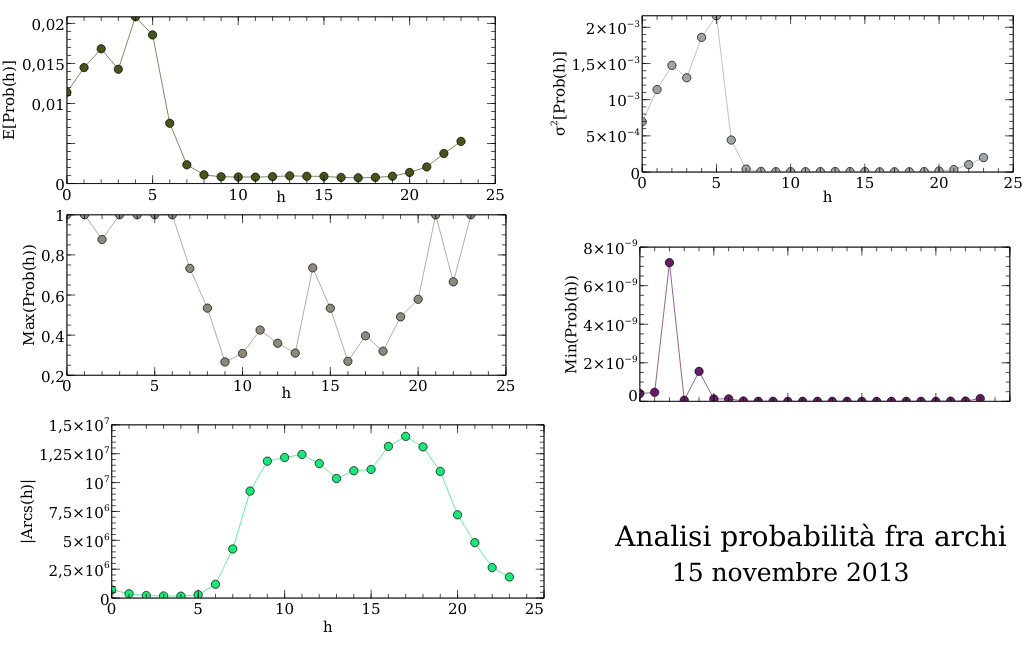
\includegraphics[scale=.6]{img/probs15nov.png}
 \caption{Statistiche sui pesi degli archi, 15 novembre. Sulle ascisse le fascie orarie. Da sinistra a destra e dal basso verso l'alto abbiamo (a)...(e)}
 \label{img:probs}
\end{figure}
Nella figura \emph{(a)} è stato evidenziata la media empirica della v.a. per ogni ora del 15 novembre. Si noti come durante la notte i valori medi siano sensibilmente più alti, a riprova del fatto che il numero di archi nella stella uscente di ogni nodo è minore in tali grafi orari. Tale ipotesi viene suffragata dal grafico mostrato in \emph{e}, in cui viene mostrato il numero di archi totali per ogni grafo orario. 

In \emph{(b)} abbiamo invece scelto di evidenziare la varianza della v.a. $Prob$. Si noti che la varianza è estremamente basse negli orari lavorativi, mostrando come in questo caso i molti archi uscenti mostrati in \emph{(e)} tendano a stabilizzarsi sul valore medio.

In \emph{(c), (d)} mostriamo invece i massimi valori assunti dagli archi su ogni grafo orario. Di particolare interesse è \emph{(c)}, da cui si nota come anche nelle ore di traffico molto elevato esistano dei picchi notevoli nei valori degli archi. I minimi rimangono sempre invece nell'ordine di $10^{-9}$, mostrando comunque un incremento considerevole, seppur in scala, nelle ore notturne.
 
\subsection{Componenti Fortemente Connesse}

Le CFC sono state disegnate su mappe (utilizzando \verb!gnuplot!) assegnando una funzione $z$ alle celle di
coordinate $(x,y)$ così definita:
$$
z(x,y) =
\begin{cases}
0, & \text{se $(x,y)$ non appartiene ad alcuna CFC,} \\
10k, & \text{se $(x,y)$ appartiene alla k-esima CFC trovata.}
\end{cases}
$$
Il valore della funzione $z$ non ha alcun significato: è stato semplicemente utilizzato al fine di assegnare differenti colori a differenti CFC; la costante $10$ è un \emph{numero magico} che consente una differenza cromatica sufficiente a poter individuare differenti CFC in maniera pressoché immediata. Si noti come i grafici disegnino unicamente le celle appartenenti a delle CFC individuate e con cardinalità maggiore di uno e lo facciano nella posizione corretta secondo la griglia di separazione definita nei dataset.

\subsubsection{SCC1}\label{scc1_0-005}
Come esempio per tutti i casi in cui l'ordine di visita dei nodi è indotto dal traffico orario, riportiamo il caso SCC1 con taglio degli archi con probabilità minore o uguale a 0.005.
In questo caso, le componenti sono per la maggior parte delle ore estremamente ampie, come si può vedere in seguito in \ref{scc1_0-005_night} \label{list:scc1_0-005} e \ref{scc1_0-005-day}. 
In particolare in \ref{scc1_0-005_night} il grafo è probabilmente composto per la maggiorparte da archi di probabilità piuttosto bassa, per cui si ottengono molto semplicemente delle CFC piuttosto distinte. Invece in \ref{scc1_0-005-day} si vede come il taglio si riveli insufficente e le componenti individuate coprano buona parte dell'area presa in considerazione. La notte il comportamento è simile a quello mostrato in figura. Alle 6 del mattino si nota invece una completa assenza di componenti, mentre dalle 8 alle 23 il comportamento è pressoché il medesimo di quello mostrato in \ref{scc1_0-005-day}.
\begin{figure}
\centering
\begin{subfigure}[b]{1\textwidth}
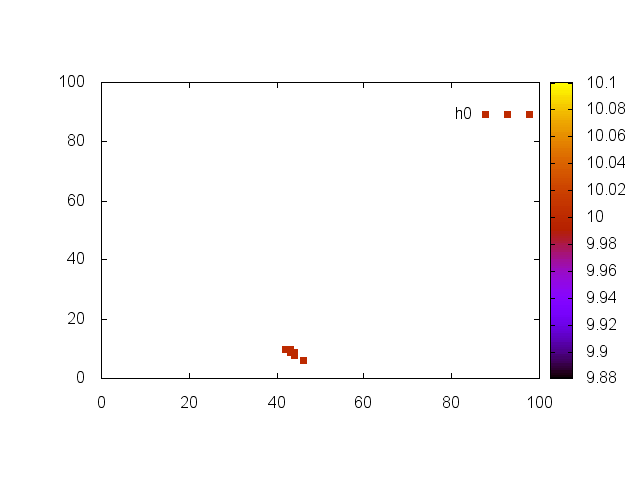
\includegraphics[scale=.5]{./img/stampe/scc1/0.png}
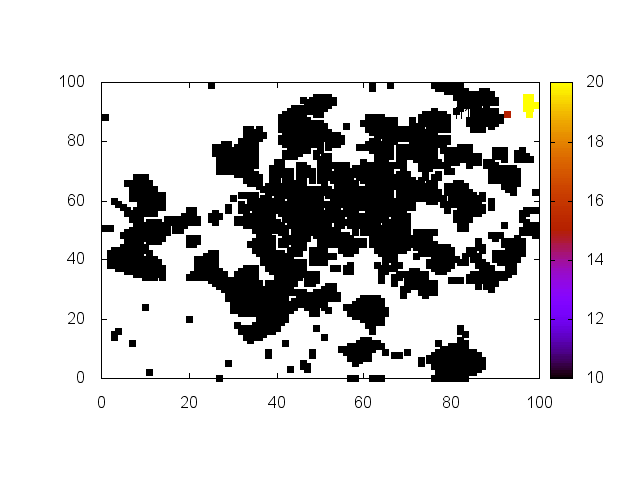
\includegraphics[scale=.5]{./img/stampe/scc1/1.png}
\end{subfigure}
\begin{subfigure}[b]{1\textwidth}
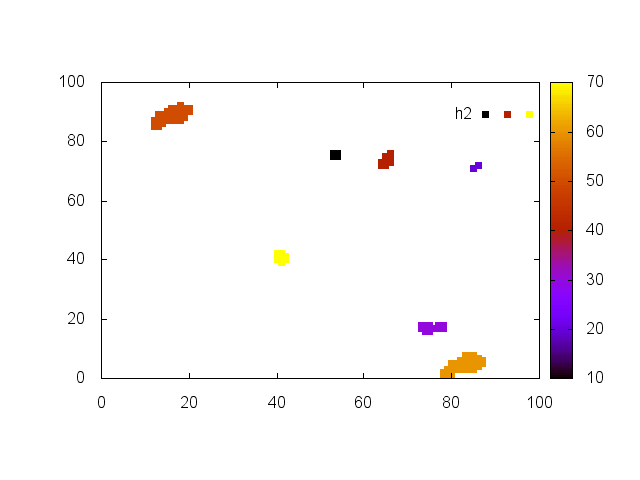
\includegraphics[scale=.5]{./img/stampe/scc1/2.png}
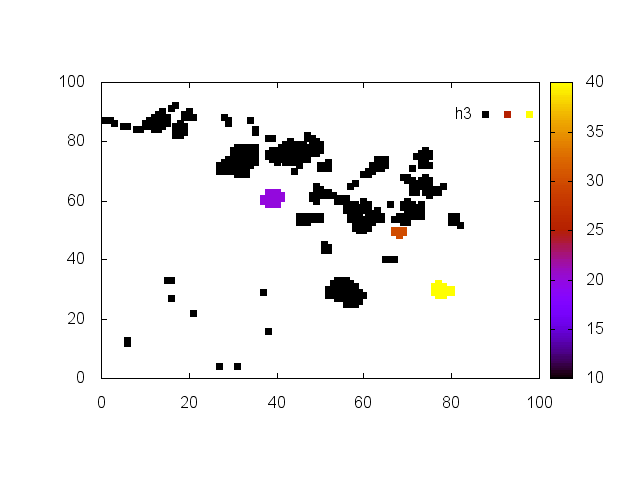
\includegraphics[scale=.5]{./img/stampe/scc1/3.png}
\end{subfigure}
\caption{comportamento nelle ore notturne (0-3) con SCC1 e taglio a 0.005}
\label{scc1_0-005_night}
\end{figure}
\begin{figure}
\centering
\begin{subfigure}[b]{1\textwidth}
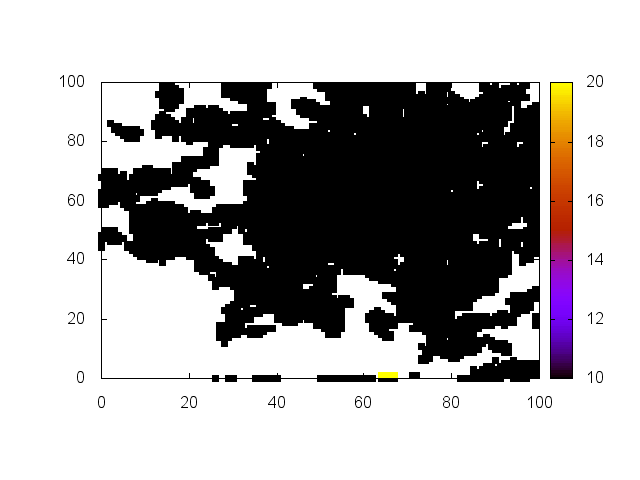
\includegraphics[scale=.5]{./img/stampe/scc1/12.png}
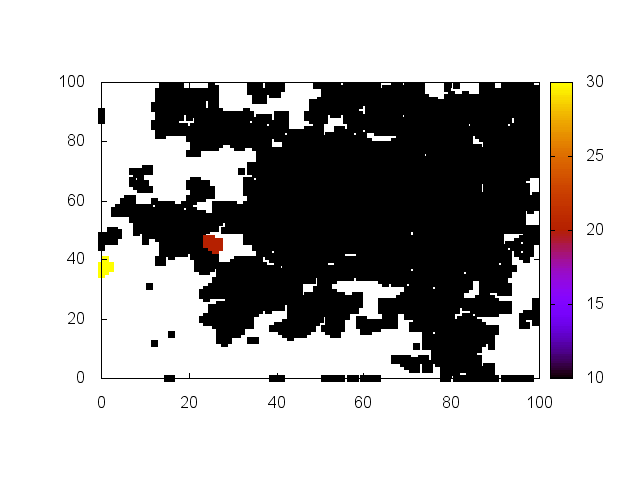
\includegraphics[scale=.5]{./img/stampe/scc1/13.png}
\end{subfigure}
\begin{subfigure}[b]{1\textwidth}
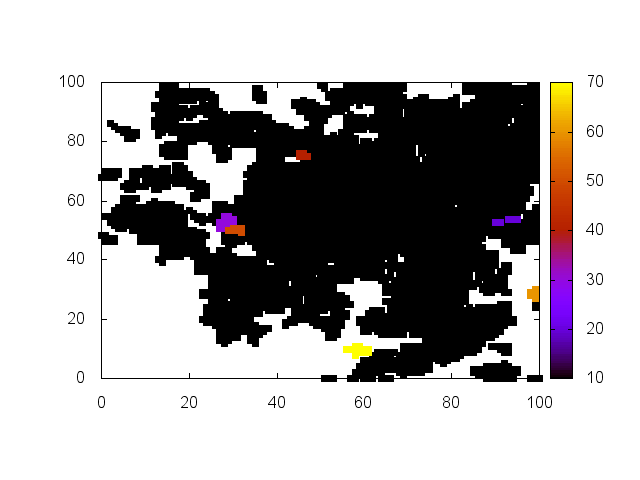
\includegraphics[scale=.5]{./img/stampe/scc1/14.png}
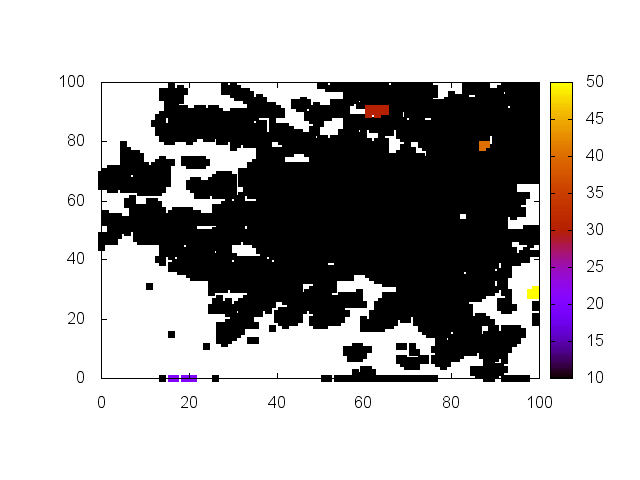
\includegraphics[scale=.5]{./img/stampe/scc1/15.png}
\end{subfigure}
\caption{comportamento nelle ore diurne (12-15) con SCC1 e taglio a 0.005}
\end{figure}
Si noti in ~\ref{list:scc1_0-005} come la dimensione delle componenti può variare anche notevolmente a seconda del traffico presente in un'ora. Questo potrebbe essere dovuto al fatto che il taglio è estremamente basso, e pertanto agisce solamente su una parte minima degli archi. Nelle ore in cui il traffico è minore, anche le componenti hanno dimensioni notevolmente minori: probabilmente questo è dovuto al fatto che il numero di archi uscenti (fuori dall'orario lavorativo) è minore e con probabilità maggiore. Questo può essere visto anche da ~\ref{img:probs}\emph{(a), (c), (e)}.
\begin{figure}
\begin{verbatim}
0:      6,
1:      2972,11,
2:      4,2,13,10,38,40,9,
3:      462,19,7,16,
4:      7,41,7,14,14,
5:      2563,2,18,
6:
7:      8010,
8:      6605,29,
9:      5677,5,8,5,
10:     5638,4,
11:     5492,4,5,3,13,6,
12:     5729,4,
13:     5692,14,11,
14:     5818,5,13,5,8,6,12,
15:     5784,5,12,3,5,
16:     5362,11,
17:     5118,9,7,15,14,5,
18:     5623,8,2,11,11,14,
19:     5951,5,5,10,
20:     6676,11,6,
21:     7449,12,
22:     7971,2,
\end{verbatim}
\caption{Nel listato, per ogni ora (alla sinistra), una lista delle dimensioni delle CFC trovate}
\label{list:scc1_0-005}
\end{figure}
Il comportamento in questo caso non è quindi stato considerato soddisfacente, visto l'eccessivo sbilanciamento nelle dimensioni delle CFC e la difficoltà di individuarne una logica o dei confini a livello geografico.
Con tagli maggiori i risultati non si rivelano differenti. In \label{scc1_0-05_night} si può vedere il comportamento notturno e in \label{scc1_0-05_day} quello diurno: 

Le componenti individuate nel taglio maggiore non sempre sono sottoinsiemi di quelle individuate in precedenza: anzi, ciò avviene in generale di rado e quando la CFC individuata ha come archi a se interna principalmente quelli con probabilità più elevata.
Come si può vedere nell'algoritmo \ref{pseudotarjan}, infatti, viene svolta una visita di profondità. I nodi inoltre possono essere visitati una sola volta e una sola volta sono considerati come possibili appartenenti a una componente fortemente connessa.

Dato il grafo senza tagli $G=(V,E)$ e sia $P:V \times V \to [0,1]$ la funzione che assegna un valore di probabilità agli archi, definiamo
$P_{cut}(u,v) =
\begin{cases}
P(u,v) & \text{se } P(u,v) > cut\\
0 	& \text{altrimenti}
\end{cases}$

Sia ora $G_{cut}=(V,E')$ il grafo tagliato, in cui $E' = \{(u,v) \in E : P_{cut}(u,v) > 0\}$. Definiamo ora la CFC ottenuta partendo da un nodo $v \in V$ come $C_{cut}( v ) = W \subseteq V. W \text{ è una CFC in } G_{cut} $. Infine sia $ T_{cut_{dfs}}(v) = T \subseteq V . T \text{ è l'insieme degli archi nell'albero generato dalla visita dfs in } G_{cut} \text{ originata in } v $ e $\alpha_{cut} (v, e) = \{ v_{0}, v_{1}, v_{2}, ... , v_{n-1}, v_{n} = e : \forall i = 0...n-1 . (v_{i}, v{i+1}) \in E' \}  \subseteq T_{cut_{dfs}}$ la sequenza di archi orientati che conduce dal nodo $v$ al nodo $e$.

Sia $a,b \in G . a < b$, dove il $<$ significa che $a$ viene visitato prima di $b$. Supponiamo inoltre che esista $C_{c_{2}}( b )$ con cardinalità maggiore di 1; sia infine $c_{1} < c_{2}$, è possibile trovare un esempio che dimostri che:
$$
\exists x \in V . \alpha_{c_{1}}(a, x) \cap C_{c_{2}}( b ) \neq  \varnothing \Rightarrow C_{c_{2}}(b) \neq C_{c_{1}}( b ) \land |C_{c_{2}}(b)| > |C_{c_{1}}(b)|
$$


In poche parole, è possibile che un taglio su un valore più basso possa reintrodurre nella ricerca delle CFC un cammino con almeno un arco il cui valore di $P$, contenuto tra $c_{1}$ e $c_{2}$, porti alla rimozione di nodi o addirittura alla disturzione della CFC individuata con un taglio su un valore maggiore. 

Nel nostro contesto, anche minime variazioni nel taglio possono reintrodurre un gran numero di cammini e questo spiega perché non sempre si possono ritrovare su tagli con valori più bassi tutte le CFC individuate con tagli su valori più alti, che sarebbero intuivitamente più selettivi.

Una possibile soluzione a questo problema potrebbe essere individuare una variazione a \ref{pseudotarjan} per cui una precedente visita di un nodo non lo  escluda successivamente dalla ricerca di ulteriori CFC, \textbf{pur mantenendo le CFC disgiunte}. In questo frangente presumibilmente la relazione di inclusione varrebbe.

%\subsection{SCC1, taglio 0.05}
%In questo caso, invece, le dimensioni delle componenti fortemente connesse diminuiscono notevolmente. Si noti, a conferma dell'ipotesi fatta in \ref{scc1_0-005}, come le dimensioni delle CFC calino drasticamente nelle ore di maggior traffico, mentre le ore che hanno un traffico inferiore sono caratterizzate da CFC più ampie.
%Si veda \ref{list:scc1_0-05}. Questo sembra indicare la necessità di effettuare tagli diversi per ore diverse, in modo da poter gestire diverse distribuzioni di traffico.
%\begin{figure}
%\begin{verbatim}
%0:      4,7,2,2,6,
%1:      383,2,4,7,7,6,6,9,5,9,2,
%2:      6,4,6,11,5,4,4x,2,8,8,
%3:      5,6,5,11,9,
%4:      6,4,8,6,6,
%5:      8,4,3,5,8,3,7,2,3,
%6:      718,4,2,10,9,3,6,3,7,3,6,7,3,
%7:      115,6,2,2,3,2,2,2,3,4,
%8:      2,3,
%9:
%10:     2,2,
%11:     2,
%12:     3,
%13:     2,
%14:
%15:     4,
%16:
%17:     2,
%18:     4,5,5,
%19:
%20:
%21:     2,2,2,2,4,5,2,5,
%22:     248,2,2,2,2,4,2,6,6,4,2,2,2,2,9,
%\end{verbatim}
%\caption{Da leggersi come in \ref{list:scc1_0-005}}
%\label{list:scc1_0-05}
%\end{figure}
%Il risultato ottenuto, anche in questo caso non è stato considerato soddisfacente. Come esempio, mostriamo in \ref{list:scc1_0-05_1011cfc} le componenti fortemente connesse trovate alle ore 10 e alle ore 11. Oltre alla loro dimensione - certamente non eccessiva - si può vedere che le CFC in 10 scompaiono in 11.
%Il dato confortante è che le CFC sono contigue geograficamente; ciò parebbe confermare l'ipotesi di una correlazione tra frequenza delle chiamate e vicinanza geografica.
%\begin{figure}
%\begin{subfigure}[b]{1\textwidth}
%\begin{verbatim}
%==== 10.cfc
%{7249,7250}
%{7724,7824}
%\end{verbatim}
%\begin{verbatim}
%====11.cfc
%{3659,3660}
%\end{verbatim}
%\end{subfigure}
%\caption{Le CFC trovate alle ore 10 e alle ore 11 del 15 Novembre 2013}
%\label{list:scc1_0-05_1011cfc}
%\end{figure}
%\subsection{SCC2, taglio 0.005}
%Il comportamento evidenziato con questo tipo di visita, che, ricordiamo, seleziona prima i nodi con minore traffico e dalla stella uscenti quelli con minore probabilità, non danno risultati estremamente diversi.
%%todo: continuare.

\subsubsection{Stable, taglio al 99-esimo percentile}


\begin{figure}
\centering

\begin{subfigure}[b]{1\textwidth}
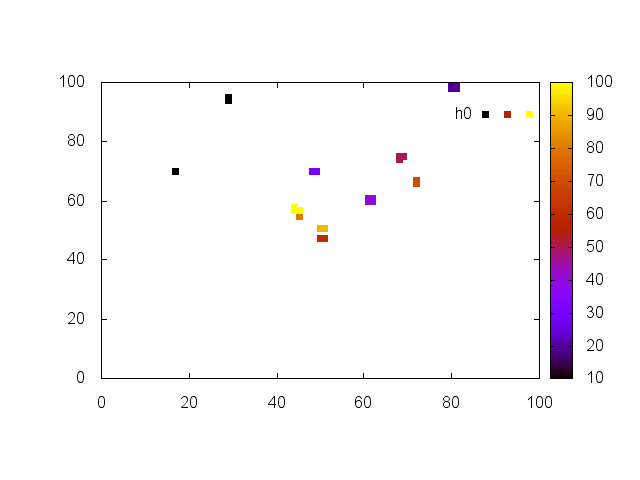
\includegraphics[scale=.3]{./img/SCC_Stable3/cut99p/0.png}
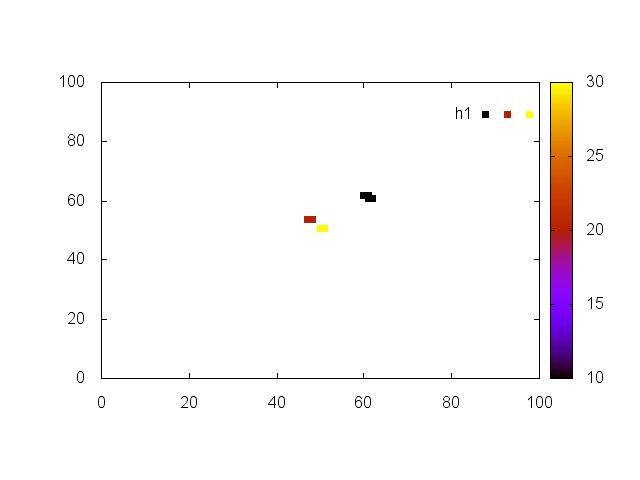
\includegraphics[scale=.3]{./img/SCC_Stable3/cut99p/1.png}
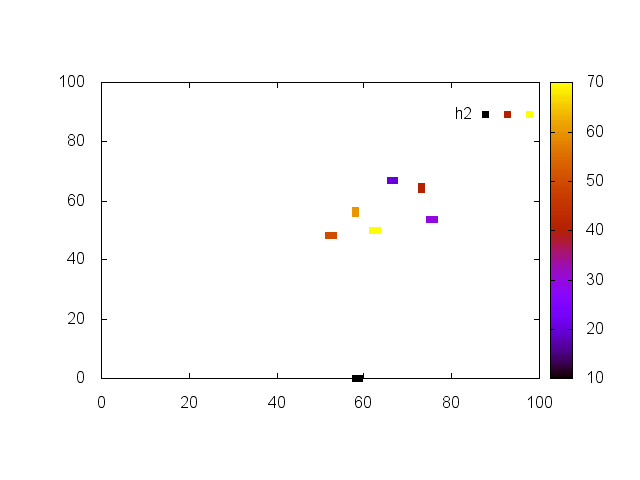
\includegraphics[scale=.3]{./img/SCC_Stable3/cut99p/2.png}
\end{subfigure}

\begin{subfigure}[b]{1\textwidth}
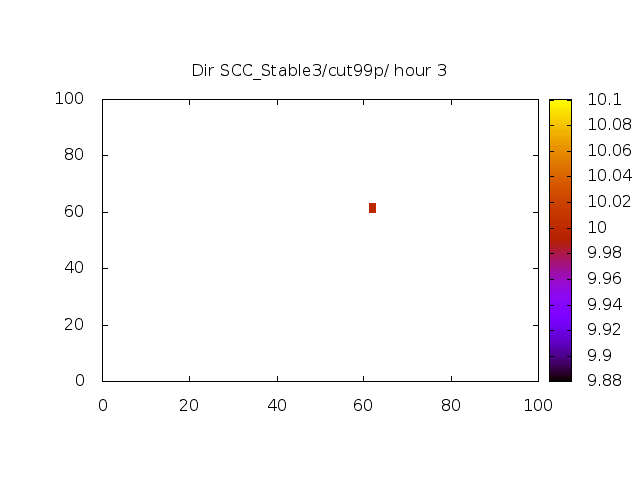
\includegraphics[scale=.3]{./img/SCC_Stable3/cut99p/3.png}
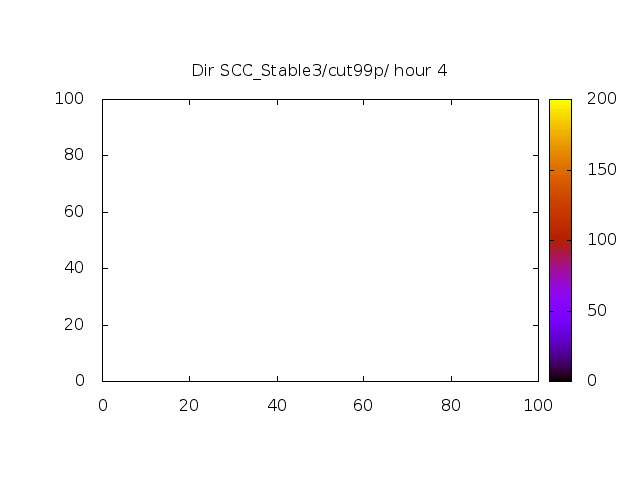
\includegraphics[scale=.3]{./img/SCC_Stable3/cut99p/4.png}
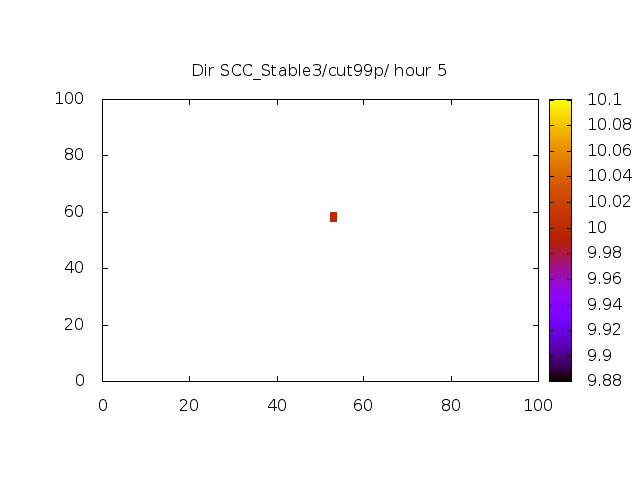
\includegraphics[scale=.3]{./img/SCC_Stable3/cut99p/5.png}
\end{subfigure}

\begin{subfigure}[b]{1\textwidth}
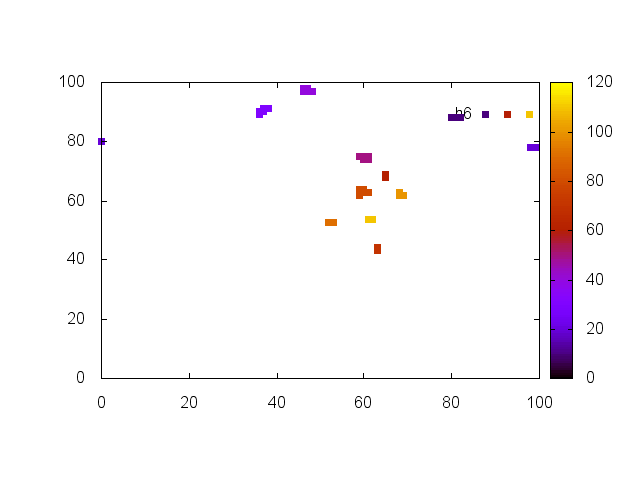
\includegraphics[scale=.3]{./img/SCC_Stable3/cut99p/6.png}
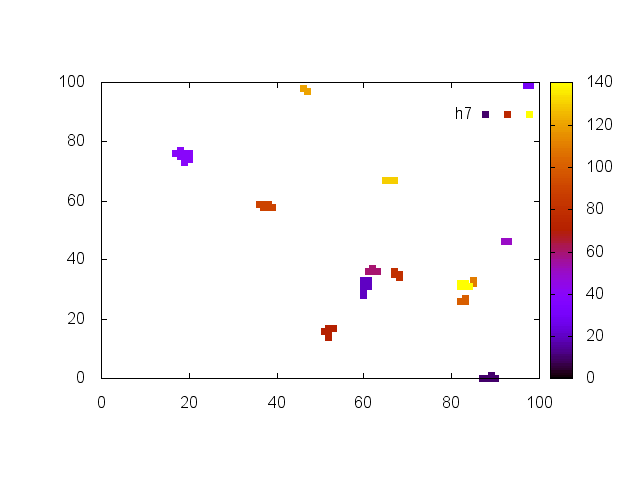
\includegraphics[scale=.3]{./img/SCC_Stable3/cut99p/7.png}
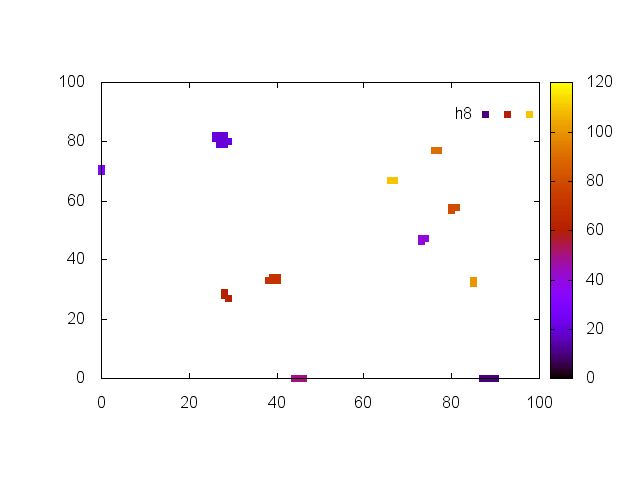
\includegraphics[scale=.3]{./img/SCC_Stable3/cut99p/8.png}
\end{subfigure}
\begin{subfigure}[b]{1\textwidth}
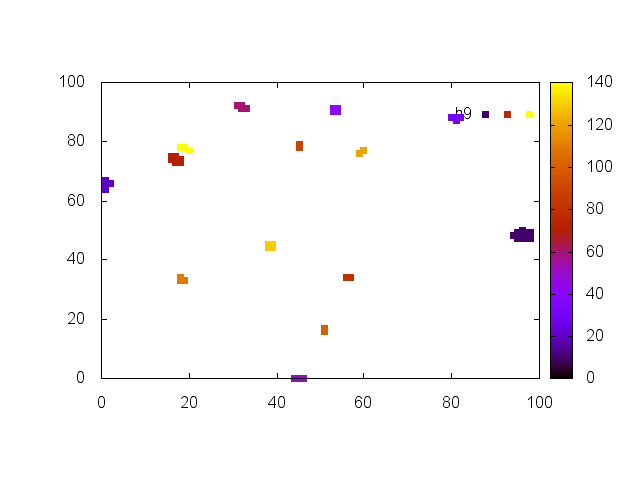
\includegraphics[scale=.3]{./img/SCC_Stable3/cut99p/9.png}
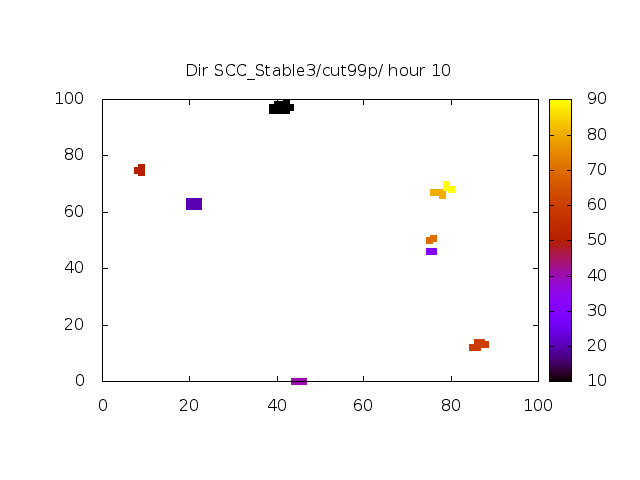
\includegraphics[scale=.3]{./img/SCC_Stable3/cut99p/10.png}
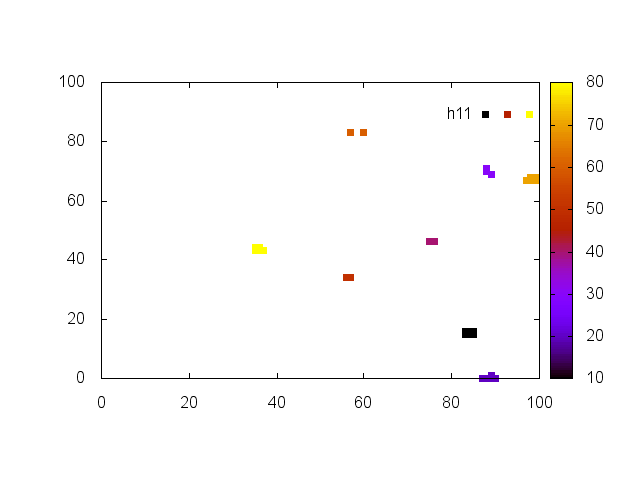
\includegraphics[scale=.3]{./img/SCC_Stable3/cut99p/11.png}
\end{subfigure}
\caption{Stable, Taglio 99-esimo percentile, h 0-11. Da vedere da sinistra verso destra e dall'alto verso il basso}
\end{figure}


\begin{figure}
\centering

\begin{subfigure}[b]{1\textwidth}
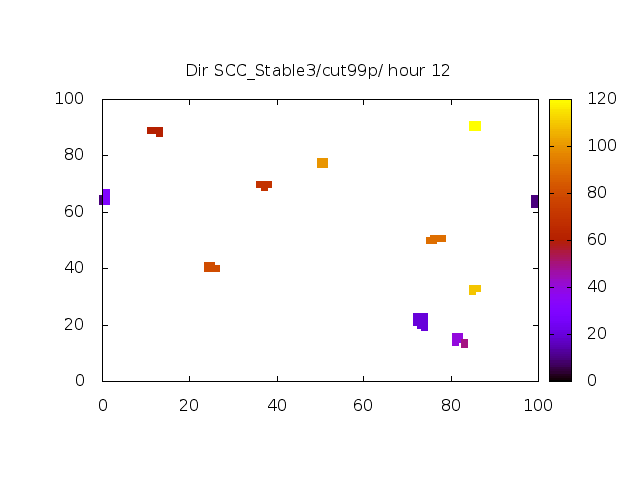
\includegraphics[scale=.3]{./img/SCC_Stable3/cut99p/12.png}
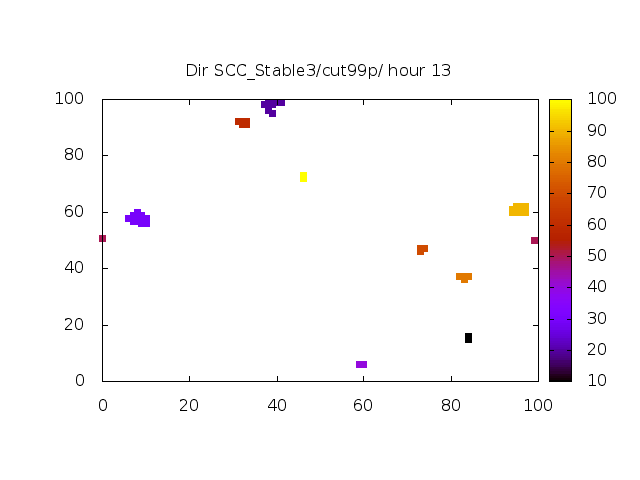
\includegraphics[scale=.3]{./img/SCC_Stable3/cut99p/13.png}
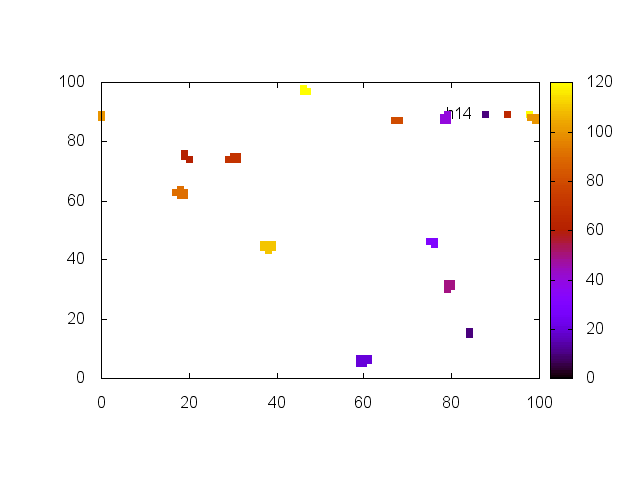
\includegraphics[scale=.3]{./img/SCC_Stable3/cut99p/14.png}
\end{subfigure}

\begin{subfigure}[b]{1\textwidth}
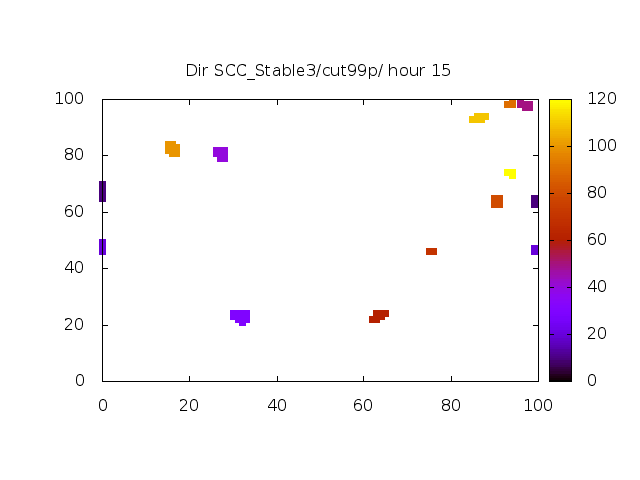
\includegraphics[scale=.3]{./img/SCC_Stable3/cut99p/15.png}
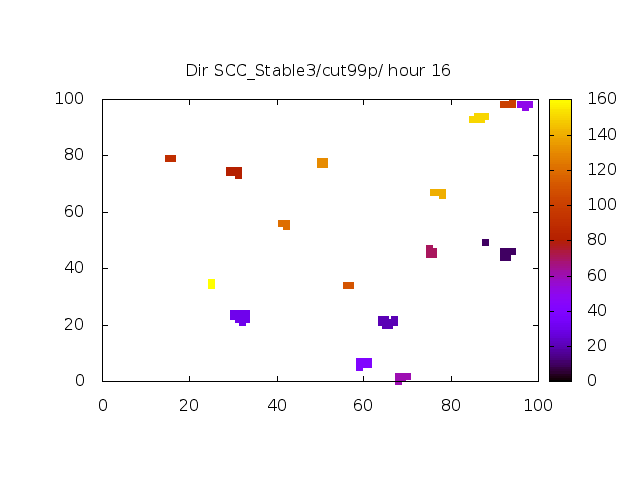
\includegraphics[scale=.3]{./img/SCC_Stable3/cut99p/16.png}
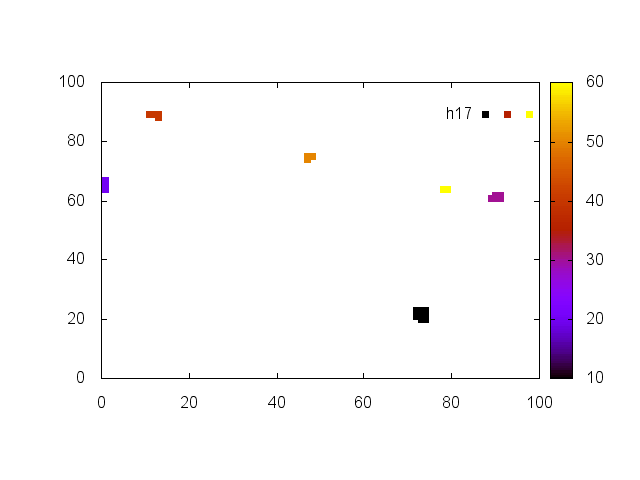
\includegraphics[scale=.3]{./img/SCC_Stable3/cut99p/17.png}
\end{subfigure}

\begin{subfigure}[b]{1\textwidth}
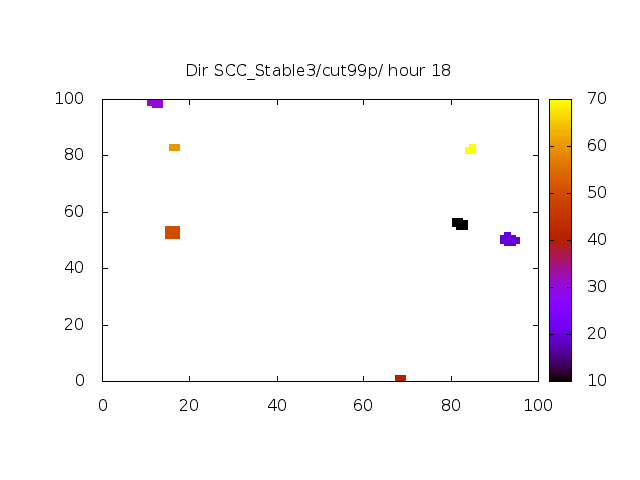
\includegraphics[scale=.3]{./img/SCC_Stable3/cut99p/18.png}
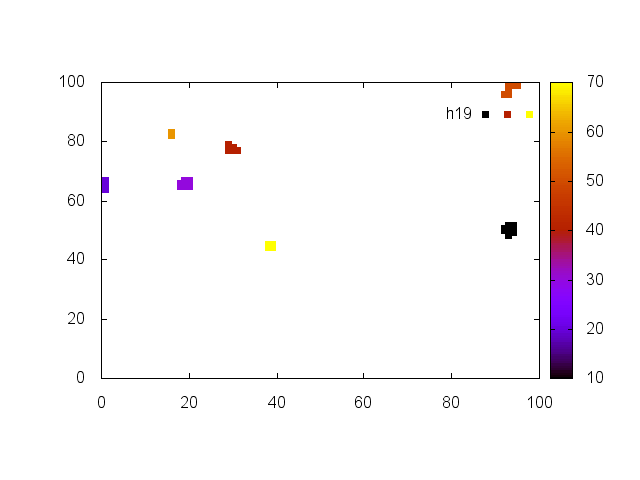
\includegraphics[scale=.3]{./img/SCC_Stable3/cut99p/19.png}
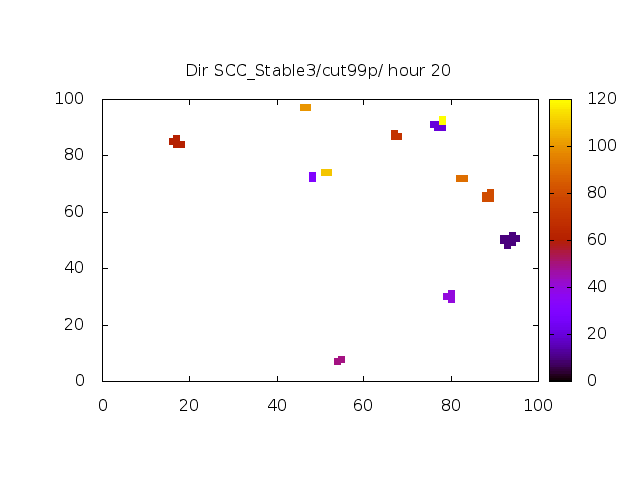
\includegraphics[scale=.3]{./img/SCC_Stable3/cut99p/20.png}
\end{subfigure}
\begin{subfigure}[b]{1\textwidth}
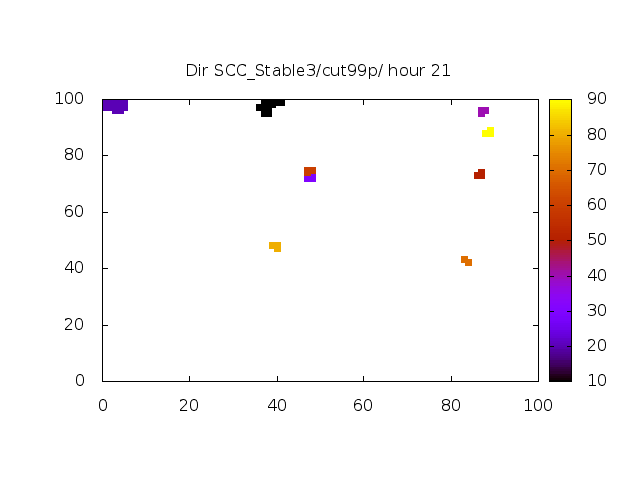
\includegraphics[scale=.3]{./img/SCC_Stable3/cut99p/21.png}
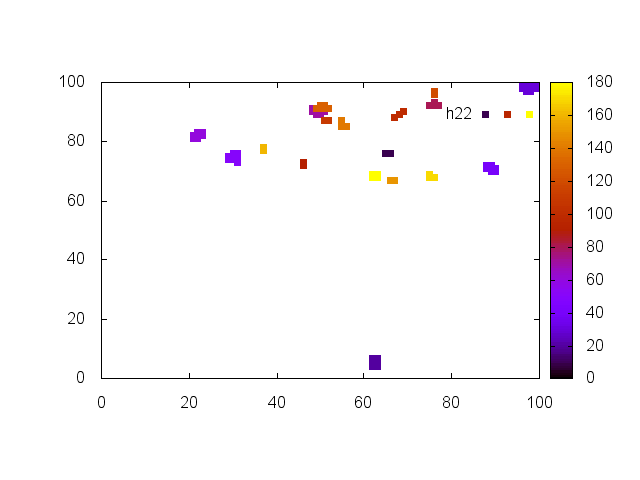
\includegraphics[scale=.3]{./img/SCC_Stable3/cut99p/22.png}
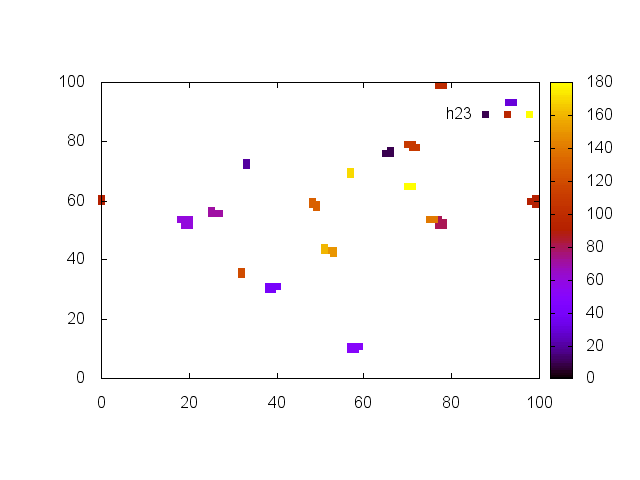
\includegraphics[scale=.3]{./img/SCC_Stable3/cut99p/23.png}
\end{subfigure}
\caption{Stable, Taglio 99-esimo percentile, h 12-23. Da vedere da sinistra verso destra e dall'alto verso il basso}
\end{figure}


\subsubsection{Stable, taglio al 95-esimo percentile}

\begin{figure}
\centering
\begin{subfigure}[b]{1\textwidth}
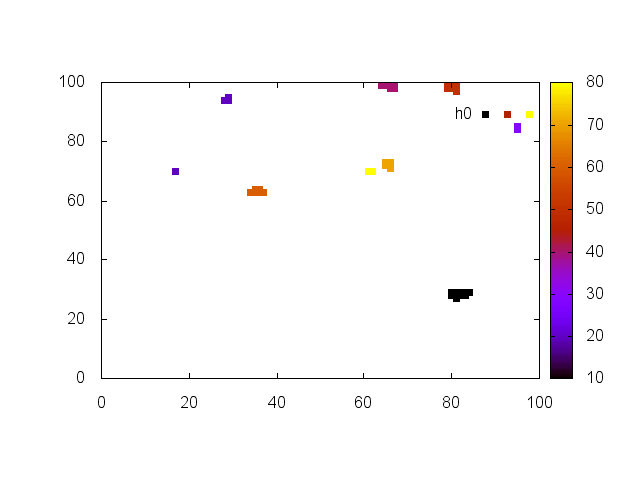
\includegraphics[scale=.3]{./img/SCC_Stable3/cut95p/0.png}
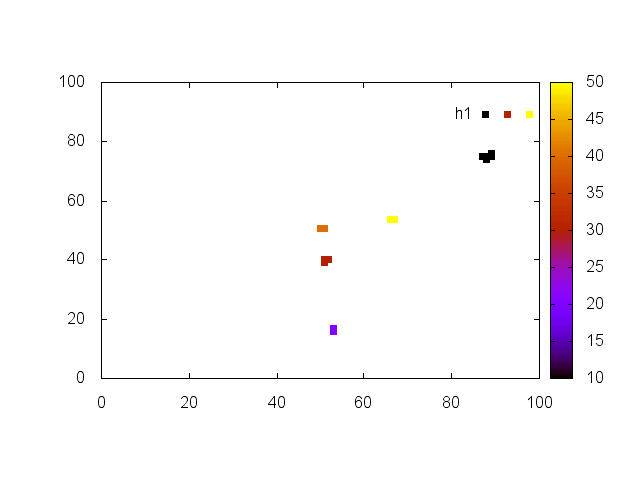
\includegraphics[scale=.3]{./img/SCC_Stable3/cut95p/1.png}
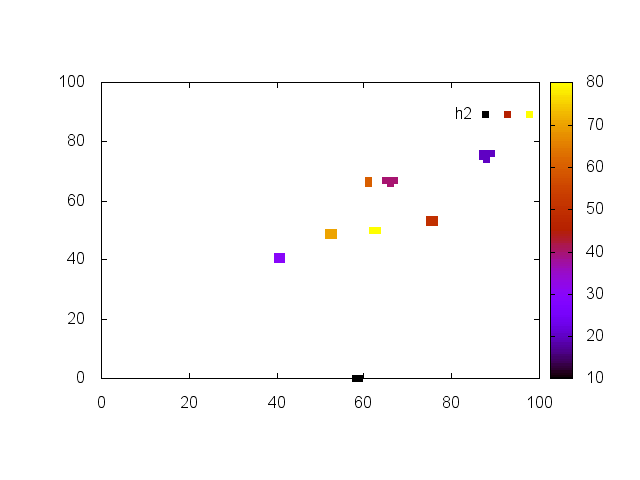
\includegraphics[scale=.3]{./img/SCC_Stable3/cut95p/2.png}
\end{subfigure}

\begin{subfigure}[b]{1\textwidth}
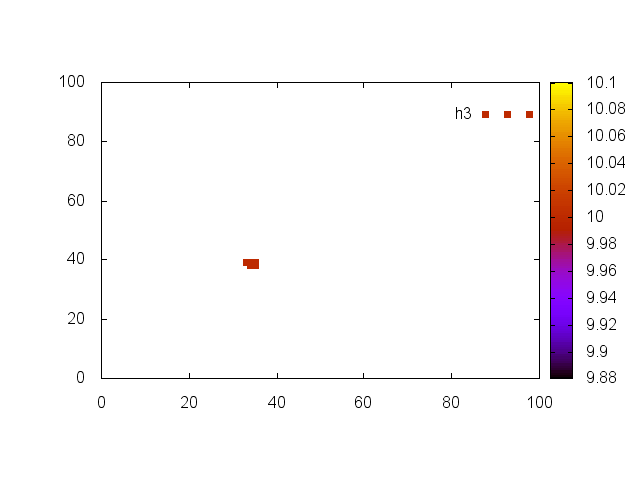
\includegraphics[scale=.3]{./img/SCC_Stable3/cut95p/3.png}
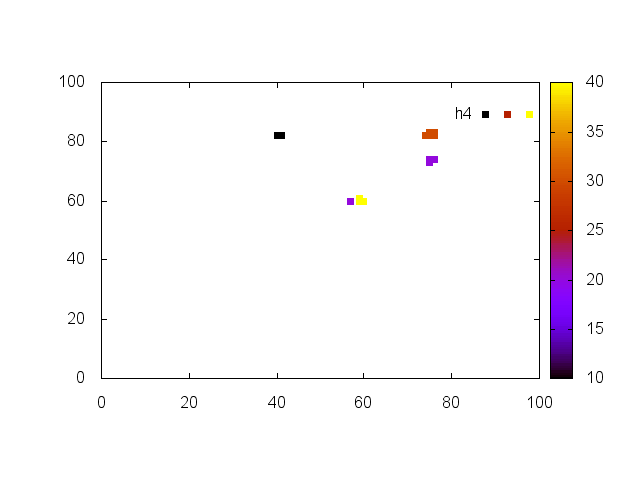
\includegraphics[scale=.3]{./img/SCC_Stable3/cut95p/4.png}
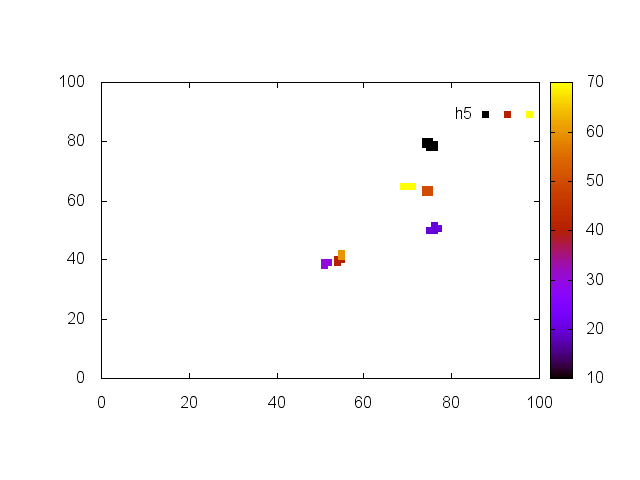
\includegraphics[scale=.3]{./img/SCC_Stable3/cut95p/5.png}
\end{subfigure}

\begin{subfigure}[b]{1\textwidth}
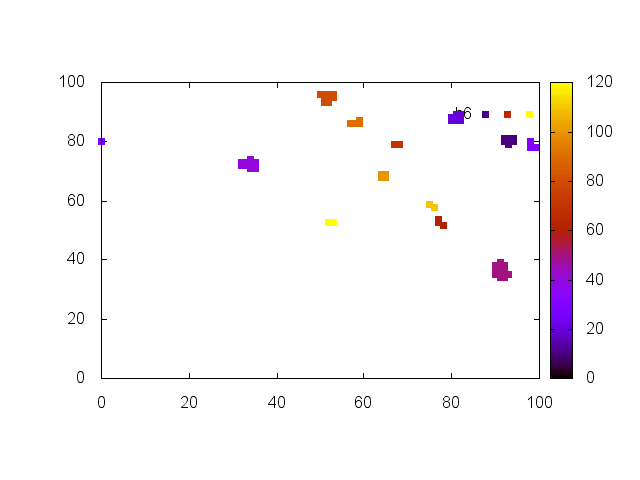
\includegraphics[scale=.3]{./img/SCC_Stable3/cut95p/6.png}
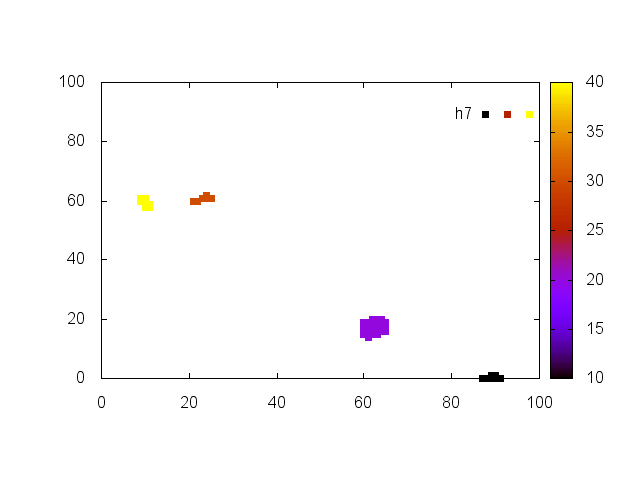
\includegraphics[scale=.3]{./img/SCC_Stable3/cut95p/7.png}
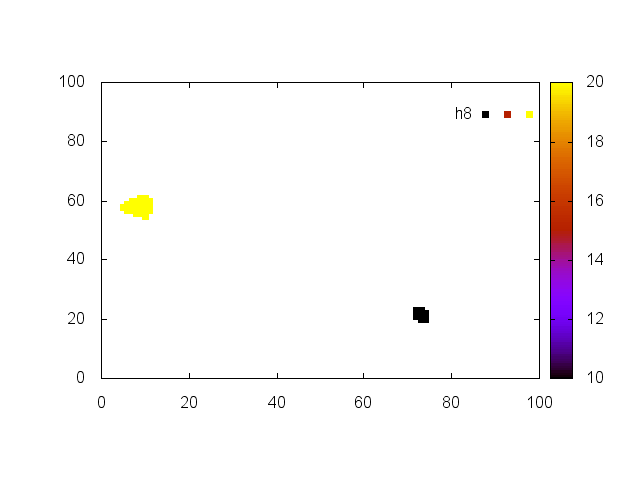
\includegraphics[scale=.3]{./img/SCC_Stable3/cut95p/8.png}
\end{subfigure}
\begin{subfigure}[b]{1\textwidth}
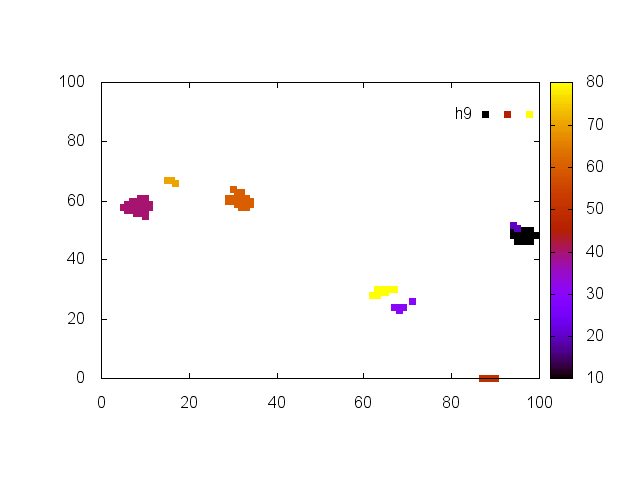
\includegraphics[scale=.3]{./img/SCC_Stable3/cut95p/9.png}
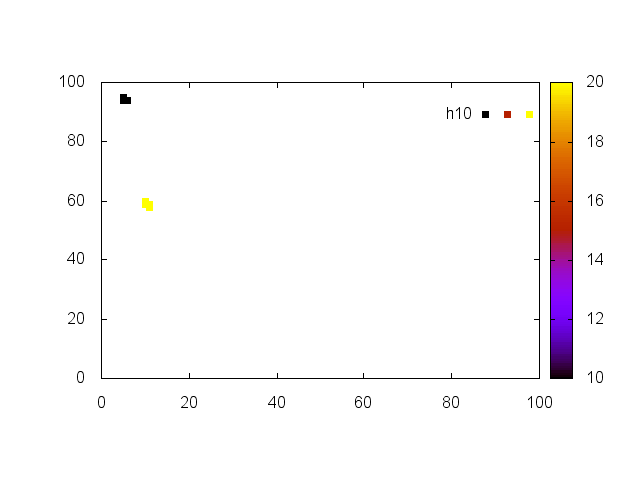
\includegraphics[scale=.3]{./img/SCC_Stable3/cut95p/10.png}
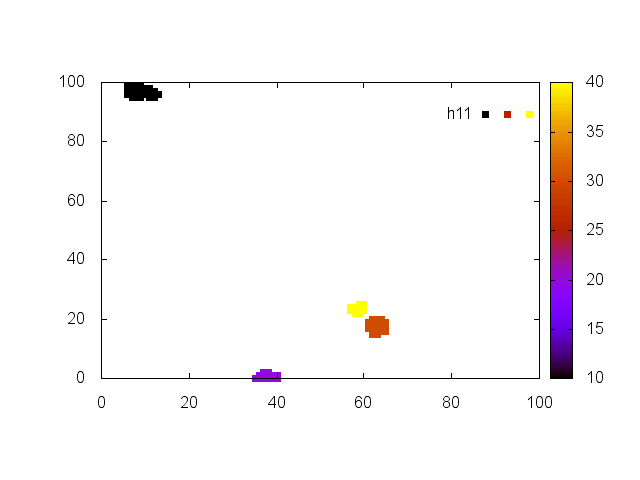
\includegraphics[scale=.3]{./img/SCC_Stable3/cut95p/11.png}
\end{subfigure}
\caption{Stable, Taglio 95-esimo percentile, h 0-11. Da vedere da sinistra verso destra e dall'alto verso il basso}
\end{figure}

\begin{figure}
\centering

\begin{subfigure}[b]{1\textwidth}
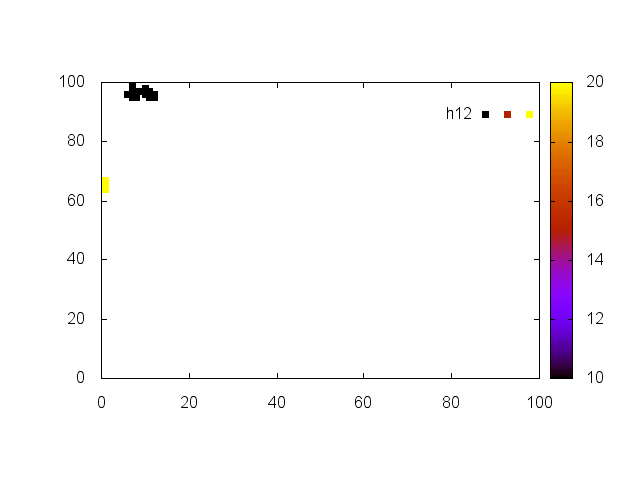
\includegraphics[scale=.3]{./img/SCC_Stable3/cut95p/12.png}
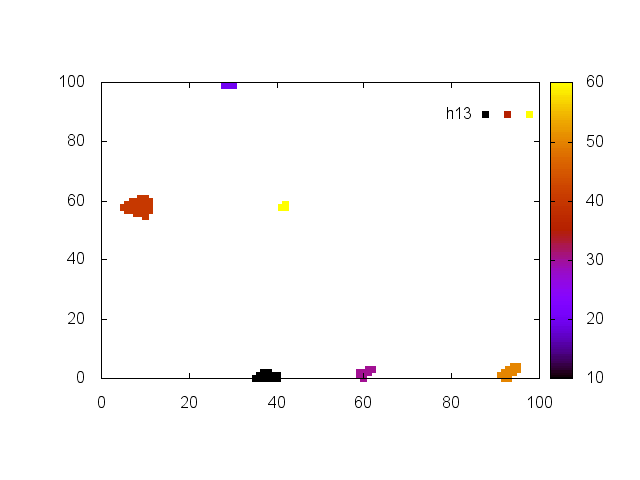
\includegraphics[scale=.3]{./img/SCC_Stable3/cut95p/13.png}
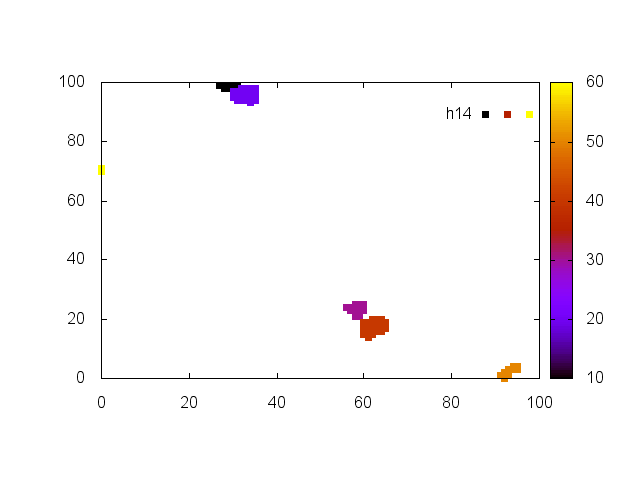
\includegraphics[scale=.3]{./img/SCC_Stable3/cut95p/14.png}
\end{subfigure}

\begin{subfigure}[b]{1\textwidth}
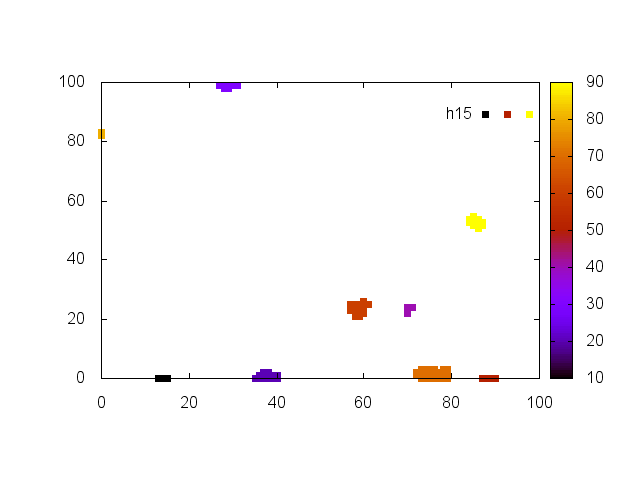
\includegraphics[scale=.3]{./img/SCC_Stable3/cut95p/15.png}
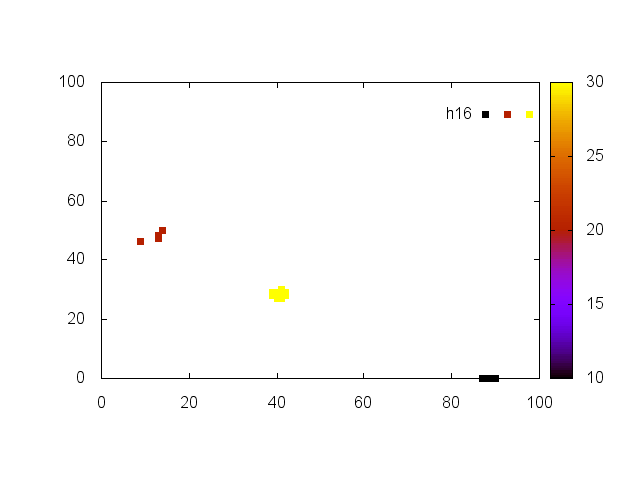
\includegraphics[scale=.3]{./img/SCC_Stable3/cut95p/16.png}
\includegraphics[scale=.3]{./img/SCC_Stable3/cut95p/17.png}
\end{subfigure}

\begin{subfigure}[b]{1\textwidth}
\includegraphics[scale=.3]{./img/SCC_Stable3/cut95p/18.png}
\includegraphics[scale=.3]{./img/SCC_Stable3/cut95p/19.png}
\includegraphics[scale=.3]{./img/SCC_Stable3/cut95p/20.png}
\end{subfigure}
\begin{subfigure}[b]{1\textwidth}
\includegraphics[scale=.3]{./img/SCC_Stable3/cut95p/21.png}
\includegraphics[scale=.3]{./img/SCC_Stable3/cut95p/22.png}
\includegraphics[scale=.3]{./img/SCC_Stable3/cut95p/23.png}
\end{subfigure}
\caption{Stable, Taglio 95-esimo percentile, h 12-23. Da vedere da sinistra verso destra e dall'alto verso il basso}
\end{figure}

\subsubsection{Stable, taglio al 90-esimo percentile}

\begin{figure}
\centering
\begin{subfigure}[b]{1\textwidth}
\includegraphics[scale=.3]{./img/SCC_Stable3/cut90p/0.png}
\includegraphics[scale=.3]{./img/SCC_Stable3/cut90p/1.png}
\includegraphics[scale=.3]{./img/SCC_Stable3/cut90p/2.png}
\end{subfigure}

\begin{subfigure}[b]{1\textwidth}
\includegraphics[scale=.3]{./img/SCC_Stable3/cut90p/3.png}
\includegraphics[scale=.3]{./img/SCC_Stable3/cut90p/4.png}
\includegraphics[scale=.3]{./img/SCC_Stable3/cut90p/5.png}
\end{subfigure}

\begin{subfigure}[b]{1\textwidth}
\includegraphics[scale=.3]{./img/SCC_Stable3/cut90p/6.png}
\includegraphics[scale=.3]{./img/SCC_Stable3/cut90p/7.png}
\includegraphics[scale=.3]{./img/SCC_Stable3/cut90p/8.png}
\end{subfigure}
\begin{subfigure}[b]{1\textwidth}
\includegraphics[scale=.3]{./img/SCC_Stable3/cut90p/9.png}
\includegraphics[scale=.3]{./img/SCC_Stable3/cut90p/10.png}
\includegraphics[scale=.3]{./img/SCC_Stable3/cut90p/11.png}
\end{subfigure}
\caption{Stable, Taglio 90-esimo percentile, h 0-11. Da vedere da sinistra verso destra e dall'alto verso il basso}
\end{figure}

\begin{figure}
\centering

\begin{subfigure}[b]{1\textwidth}
\includegraphics[scale=.3]{./img/SCC_Stable3/cut90p/12.png}
\includegraphics[scale=.3]{./img/SCC_Stable3/cut90p/13.png}
\includegraphics[scale=.3]{./img/SCC_Stable3/cut90p/14.png}
\end{subfigure}

\begin{subfigure}[b]{1\textwidth}
\includegraphics[scale=.3]{./img/SCC_Stable3/cut90p/15.png}
\includegraphics[scale=.3]{./img/SCC_Stable3/cut90p/16.png}
\includegraphics[scale=.3]{./img/SCC_Stable3/cut90p/17.png}
\end{subfigure}

\begin{subfigure}[b]{1\textwidth}
\includegraphics[scale=.3]{./img/SCC_Stable3/cut90p/18.png}
\includegraphics[scale=.3]{./img/SCC_Stable3/cut90p/19.png}
\includegraphics[scale=.3]{./img/SCC_Stable3/cut90p/20.png}
\end{subfigure}
\begin{subfigure}[b]{1\textwidth}
\includegraphics[scale=.3]{./img/SCC_Stable3/cut90p/21.png}
\includegraphics[scale=.3]{./img/SCC_Stable3/cut90p/22.png}
\includegraphics[scale=.3]{./img/SCC_Stable3/cut90p/23.png}
\end{subfigure}
\caption{Stable, Taglio 90-esimo percentile, h 12-23. Da vedere da sinistra verso destra e dall'alto verso il basso}
\end{figure}

\section{Alcune conclusioni}

\begin{enumerate}
\item Occorre effettuare tagli con valore molto alto perchè il grafo è inerentemente fortemente connesso.
\item Le statistiche sulle probabilità degli archi denotano l'effettiva esistenza di square che si chiamano
più degli altri negli orari non lavorativi.
\item La strategia di visita incide molto nella formazione del risultato e probabilmente il problema di
non considerare mai due volte lo stesso nodo può eliminare delle CFC interessanti.
\item Il numero di CFC è più basso di quello attesa, tuttavia le CFC sono ben distribuite spazialmente 
sulla grid; si noti anche come al variare delle fasce orarie variano le zone in cui vengono scoperte
le CFC.
\item Sopratutto nelle ore di minor traffico si individuano principalmente CFC che potrebbero essere
fatte risalire alla presenza di paesi della periferia di Milano (la grid copre un'area molto più grande
della sola zona urbana di Milano).
\item Le CFC trovate non mostrano persistenza (salvo rare eccezioni) in fasce orarie contigue ma tendono
ad apparire e scomparire. Si noti come questo non può essere dovuto al valore del taglio, perchè
i percentili vengono calcolati per ogni fascia oraria.
\end{enumerate}

\section{Prosecuzione del lavoro}

\begin{enumerate}
\item Implementazione di tutta l'analisi su Hadoop.
\item Cercare le  componenti debolmente connesse.
\item Strategie di clustering.
\item Ampliare il periodo analizzato per includere tutti i giorni di novembre e dicembre (da decidere
come aggregare i risultati giornalieri)
\item affinare il periodo di aggregazione? (e.g. passare a fasce di 30 min)
\end{enumerate}

\end{document}
